\documentclass{beamer}
\usepackage{geometry}
\usepackage[english]{babel}
\usepackage[utf8]{inputenc}
\usepackage{amsmath}
\usepackage{amsfonts}
\usepackage{amssymb}
\usepackage{tikz}
\usepackage{graphicx}
\usepackage{venndiagram}

%\usepackage{pgfplots}
%\pgfplotsset{width=10cm,compat=1.9}
%\usepackage{pgfplotstable}

\setlength{\headheight}{26pt}%doesn't seem to fix warning

\usepackage{fancyhdr}
\pagestyle{fancy}
\fancyhf{}

%\rhead{\small{5 September 2018}}
\lhead{\small{BECA / Dr. Huson / 11.1 IB Math Unit 1}}

\renewcommand{\headrulewidth}{0pt}

\title{Mathematics Class Slides}
\subtitle{Bronx Early College Academy}
\author{Chris Huson}
\date{13-17 September 2021}

\begin{document}
\frame{\titlepage}
\section[Outline]{}
\frame{\tableofcontents}


\section{1.1 1st day of Geometry, Segment addition, 13 Sept}
\frame
{
  \frametitle{Learning Target: I can measure and diagram my world}
  \framesubtitle{CCSS: HSG.CO.A.1 Know precise geometric definitions \hfill \alert{1.1 Monday 13 Sept}}

  Welcome back to school
  \begin{block}{Do Now: Measurement}
  \begin{enumerate}
      \item Notebook first page: Name / Course / Instructor
      \item Diagram people closest to you and their distance
      \item Early finishers: Calculate diagonal distances
  \end{enumerate}
  \end{block}
  Supply list: Composition book, looseleaf, pencils \& pens, \\*
  compass and ruler; Optional: calculator, folder \\[0.25cm]
  Lesson: Linear functions, slope, solving; vertical line test p 4-6 \\[0.25cm]
  Homework: Diagram your bedroom (with measurements), or another room
}

%Prepare copies of formula sheets

  \section{1.2 Function domain and range}
  \frame
  {
    \frametitle{Learning Target: I can apply domain and range}
    \framesubtitle{CCSS: HSF.IF.C.7 Analyze functions \hfill \alert{1.2 Tuesday 14 Sept}}

    \begin{block}{Do Now: In your notebook}
    \begin{enumerate}
      \item Solve for $x$: \\
      \hspace{1cm} $x-7=11$ \hspace{1cm}  $2(x-5) \geq 4$
      \item What is the slope of the line $y=3x-2$?
      \item $f(x) = x^2 - 3$. Find $f(1)$
    \end{enumerate}
    \end{block}
    Lesson: Domain, range, function review pp 204-8\\[5pt]
    Groupwork: Investigation 1 pp 206-8\\[5pt]
    Homework: Skills Check p 205
  }

  \section{1.5 Problem sets working with functions}
  \frame
  {
    \frametitle{Learning Target: I can employ the language of functions}
    \framesubtitle{CCSS: HSF.IF.C.7 Analyze functions \hfill \alert{1.5 Monday 20 Sept}}

    \begin{block}{Do Now: In your notebook}
    \begin{enumerate}
      \item Solve for $x$: \\
      \hspace{1cm} $2x-9=3$ \hspace{1cm}  $3(x-3) \leq 12$
      \item What is the slope of the line $y=2x-5$?
      \item $f(x) = x^2 +6$. Find $f(2)$
    \end{enumerate}
    \end{block}
    Lesson: Independent and dependent variables\\[5pt]
    Linear equations and function review pp 204-8\\[5pt]
    Groupwork: Exercises 5C pp 220-221\\[5pt]
  }

  \section{1.6 Problem sets working with functions}
  \frame
  {
    \frametitle{Learning Target: I can use functions to model situations}
    \framesubtitle{CCSS: HSF.IF.C.7 Analyze functions \hfill \alert{1.6 Tuesday 21 Sept}}

    \begin{block}{Do Now: Pyramid lifting routine problem 
      (\href{https://www.bodybuilding.com/content/build-muscle-and-strength-with-pyramid-training.html}{Bill Geiger})}
      \begin{center}
          Set 1: 135 lbs, 15 reps\\
          Set 2: 185 lbs, 12 reps\\
          Set 3: 205 lbs, 10 reps\\
          Set 4: 225 lbs, 8 reps\\
          Set 5: 245 lbs, 6 reps\\
          Set 6: 265 lbs, 4 reps
    \end{center}
    \end{block}
    \begin{enumerate}
      \item On the third set, when $x=3$, how much weight is lifted?
      \item On which set is the weight 245 pounds?
      \item Interpret the ordered pair $(2,185)$ in this context.
      \item Does the weight increase by a constant amount with each set?
    \end{enumerate}
    Prequiz handout; 
    Function review pp 204-220
  }

  \section{1.7 Do Now Quiz functions}
  \frame
  {
    \frametitle{Learning Target: I can use functions to model situations}
    \framesubtitle{CCSS: HSF.IF.C.7 Analyze functions \hfill \alert{1.7 Wednesday 22 Sept}}

    \begin{block}{Do Now Quiz}

    \end{block}
    \begin{enumerate}
      \item On the third set, when $x=3$, how much weight is lifted?
      \item On which set is the weight 245 pounds?
      \item Interpret the ordered pair $(2,185)$ in this context.
      \item Does the weight increase by a constant amount with each set?
    \end{enumerate}
    Review simplifying radicals, solving equations with fractions\\
    Function review pp 204-220 \\
    \alert{Test Friday on functions}
  }

  \section{1.8 PreTest review functions}
  \frame
  {
    \frametitle{Learning Target: I can use functions to model situations}
    \framesubtitle{CCSS: HSF.IF.C.7 Analyze functions \hfill \alert{1.8 Thursday 23 Sept}}

    \begin{block}{Do Now: Algebra warmup problems}
      Given the linear function $f(x)=-2x+12$
      \begin{enumerate}
        \item Find $f(0)$ \hspace{3cm}
        2. $f(x)=0$. Find $x$.
    \end{enumerate}
    \end{block}\vspace{3cm}
    Function review pp 204-220.
    \alert{Test tomorrow on functions}
  }

  \section{1.9 Linear models}
  \frame
  {
    \frametitle{Learning Target: I can use linear equations to model situations}
    \framesubtitle{CCSS: HSF.IF.C.7 Analyze functions \hfill \alert{1.9 Monday 27 Sept}}

    \begin{block}{Do Now: Investigation 5 page 221}
        Answer questions 1, 2, and 3 (including the table on page 222)
    \end{block}\vspace{3cm}
    Function test makeup: Sabrina, Qwaa, Sthefani.\\[0.5cm]
    Groupwork: problems 5D page 225-6
  }

  \section{1.9 Linear models}
  \frame
  {
    \frametitle{I can use linear equations to model situations}
    \framesubtitle{Investigation 5 page 221 \hfill \alert{1.9 Monday 27 Sept}}

    \begin{block}{Linear functions:}\vspace{0.5cm}
       $f(x)=2x+1$\\[1cm]
       $g(x)=-3x+2$\\[1cm]
       $h(x)=3$
    \end{block}\vspace{1.5cm}
  }

  \section{1.10 Linear models}
  \frame
  {
    \frametitle{Learning Target: I can use linear equations to model situations}
    \framesubtitle{CCSS: HSF.IF.C.7 Analyze functions \hfill \alert{1.10 Tuesday 28 Sept}}

    \begin{block}{Do Now: Example 6 page 222}
        Compare the two linear models (d) and (e). (formulas page 222)
        \begin{enumerate}
          \item Which has the greater rate of change?
          \item Which has the higher initial value?
        \end{enumerate}
    \end{block}\vspace{0.5cm}
    Function test makeup: Sthefani.\\[0.5cm]
    Lesson: Calculating rate of change (slope or gradient)\\[0.25cm]
    Variables and parameters
    Groupwork: problems 5D page 225-6
  }

  \section{1.11 Linear models}
  \frame
  {
    \frametitle{Learning Target: I can use linear equations to model situations}
    \framesubtitle{CCSS: HSF.IF.C.7 Analyze functions \hfill \alert{1.11 Wednesday 29 Sept}}

    \begin{block}{Do Now: Calculate your mastery score Functions}
        Let $x$ be the number of points correct on \#1-8
        \begin{enumerate}
          \item $\displaystyle f(x)=\frac{x}{10} + 0.33$
          \item $max(1,min(4,f(x)))$
        \end{enumerate}
    \end{block}\vspace{0.5cm}
    Function test review, test corrections due Monday\\[0.5cm]
    Lesson: Calculating rate of change (slope or gradient)\\[0.25cm]
    Variables and parameters
    Groupwork: problems 5D page 225-6
  }

  \frame
  {
    \frametitle{Functions mastery score (problems  \#1-8)}

    \begin{block}{Let $x$ be the number of points}
      
      \begin{enumerate}
        \item $\displaystyle f(x)=\frac{x}{10} + 0.33$
        \item $max(1,min(4,f(x)))$
        \item Example, 25 points $\displaystyle f(25)=\frac{25}{10} + 0.33=2.8$
      \end{enumerate}
    \end{block}
    IB test scoring, points:
    \begin{enumerate}
      \item ``A1'' - correct/Accurate value
      \item ``M1'' - proper Method used
      \item  ``R1'' - good Reasoning
      \item  ``N1'' - No work, but partial credit
      \item  ``ft'' - correct, but Following Through on previous errors
    \end{enumerate}
  }

  \section{1.12 Linear models}
  \frame
  {
    \frametitle{Learning Target: I can use linear equations to model situations}
    \framesubtitle{CCSS: HSF.IF.C.7 Analyze functions \hfill \alert{1.12 Thursday 30 Sept}}

    \begin{block}{Do Now: Textbook example page 222}
    \end{block}\vspace{0.5cm}
    Lesson: Calculating rate of change (slope or gradient)\\[0.25cm]
    Variables and parameters
    Groupwork: problems 5D page 225-6
  }

  \section{1.13 Direct variation}
  \frame
  {
    \frametitle{Learning Target: I can use direct variation as a model}
    \framesubtitle{CCSS: HSF.IF.C.7 Analyze functions \hfill \alert{1.13 Friday 1 Oct}}

    \begin{block}{Do Now: A linear function is such that $f(1)=5$ and $f(5)=1$.}
      \hspace{8cm} (\#7 page 225)
      \begin{enumerate}
        \item Name two of the function's points as ordered pairs.
        \item Find the gradient (slope) for the function $f$ 
      \end{enumerate}
    \end{block}\vspace{0.25cm}
    Lesson: Direct variation, constant of proportionality, IB formulas\\
    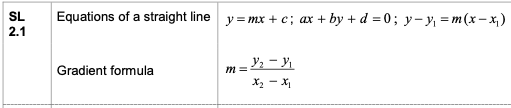
\includegraphics[width=10cm]{IB-formula-lines.png}\\
    Groupwork: problems 5E page 228
  }

\end{document}
